\section{Derivatives}
\subsection{Introduction to Derivatives}

There are three ideas at the core of calculus. We've already covered one so far, the limit, and you've all (mostly) survived so now we can move on to the derivative. Here's the problem: slopes of lines is easy, take any two points and use the slope formula. But if I point to some point on a quadratic and ask you to give me the slope then you're shit out of luck. Luckily with the power of god and \st{anime} limits on your side, we can rectify this issue (in just a few more pages too!).

To begin, what exactly does the slope at a single point mean. We can easily find the slope between two points by drawing a line between them, but for a curve there's no lines. For the case of a curve, the slope at a single point will be the slope of line which \emph{just barely} touches the curve at that point. In other words we want the slope of the tangent line of the curve at that point. But to find the slope of a tangent line, we must first discuss secant lines.

As opposed to tangent lines, we get a secant line by taking two points on a curve and drawing a line through them. For instance if we have the function $f(x) = x^2$ and we want the secant line through $x = 1$ and $x = 3$, then the slope is
\[ m = \frac{f(3) - f(1)}{3 - 1} = \frac{9 - 1}{2} = 4 \]
We can make this equation much more general:

\begin{definition}[Difference Quotient]
	Let $f$ be a function which is defined (i.e. exists) on some interval. Let $x$ be some point inside that interval and $h \neq 0$ a number such that $x + h$ is still in the interval. Then the difference quotient is
	\[ Q = \frac{f(x + h) - f(x)}{h} \]
\end{definition}

A geometrical interpretation of this equation is that it is the slope of the secant line through $x$ and the point $h$ away. If we want to get the slope of the tangent line, then we simply move that second point closer and closer to the first point. In other words, we take the limit as $h$ (the horizontal distance between the two points of the secant line) goes to 0.

In the figure below, we see graphically how we can get to a tangent line by first taking a secant line and then decreasing the distance between the two points until they converge to just one. This will give a visualization for the actual definition of a derivative which represents this idea using a limit.

\begin{center}
	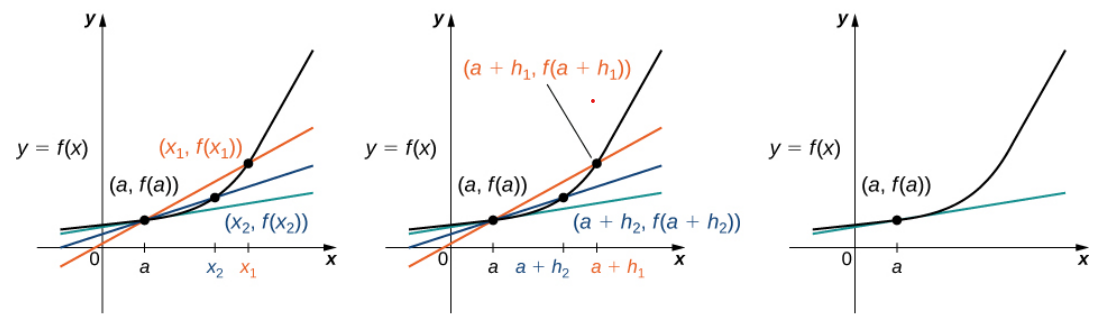
\includegraphics[scale=0.55]{images/Figure 3.1.1.png}
\end{center}

\begin{definition}[Derivatives]
	Let $f$ be a function which is defined on some open interval and $a$ some number in that interval (open interval means that $a$ cannot be either endpoint). Then the derivative of $f$ at $a$, or the slope of the tangent line at $x = a$, is given by the limit
	\[ f'(a) = \lim_{h \to 0} \frac{f(a + h) - f(a)}{h} \] 
\end{definition}

\begin{example}
	Let take perhaps the simplest example (asides from constants) known to man, a linear function
	\[ f(x) = x \]
	Then the derivative, the slope of the tangent line, at any point $x = a$ is
	\[ f'(a) = \lim_{h \to 0} \frac{(a + h) - a}{h} = \lim_{h \to 0} \frac{h}{h} = \lim_{h \to 0} 1 = 1 \]
	This makes sense because the tangent line to a line is the line itself and the slope of a line does not change.
\end{example}

\begin{example}
	Here's a more complicated example
	\[ f(x) = x^2 \]
	Again we'll be general and consider any point $x = a$.
	\begin{align*}
		f'(a) &= \lim_{h \to 0} \frac{(a + h)^2 - a^2}{h} = \lim_{h \to 0} \frac{a^2 + 2ah + h^2 - a^2}{h} \\
		&= \lim_{h \to 0} \frac{2ah + h^2}{h} = \lim_{h \to 0} 2a + h \\
		&= 2a
	\end{align*}
	So the slope of a tangent line at some $x$ value is two times that $x$ value.
\end{example}

\newpage 
\begin{example}
	One more example
	\[ f(x) = \sqrt{x} \]
	This limit is slightly more involved
	\begin{align*}
		f'(a) &= \lim_{h \to 0} \frac{\sqrt{a + h} - \sqrt{a}}{h} \\
		&= \lim_{h \to 0} \frac{a + h - a}{h (\sqrt{a + h} + \sqrt{a}} = \lim_{h \to 0} \frac{h}{h(\sqrt{a + h} + \sqrt{a}} \\
		&= \lim_{h \to 0} \frac{1}{\sqrt{a + h} + \sqrt{a}} = \frac{1}{\sqrt{a} + \sqrt{a}} \\
		&= \frac{1}{2 \sqrt{a}}
	\end{align*}
\end{example}

Sometimes you might hear a derivative referred to as an \emph{instantaneous rate of change}, this comes from physics where the slope of something represents its rate of change. With this in mind, let's do a couple more examples but set in the real world.

\begin{example}
	Suppose we chuck a ball into the air such that its height is given by
	\[ y(t) = -5t^2 + 10t \]
	We want to know exactly how fast the ball is falling when it hits the ground, so first we solve for the time when it does hit the ground.
	\[ y(t) = -5t(t - 2) = 0 \thus t = 0, 2 \]
	$t = 0$ is when we first yeet the ball, so $t = 2$ is when it comes back down. Now we can do the limit
	\begin{align*}
		v(t) &= \lim_{h \to 0} \frac{(-5(2 + h)^2 + 10(2 + h)) - (-5(2)^2 + 10(2))}{h} \\
		&= \lim_{h \to 0} \frac{-5(4 + 4h + h^2) + 20 + 10h - 0}{h} \\
		&= \lim_{h \to 0} \frac{-10h - 5h^2}{h} = \lim_{h \to 0} -10 - 5h \\
		&= -10
	\end{align*}
	For that have done some physics before may notice that I set up this problem such that we throw the ball up in the air with speed $\SI{10}{m/s}$ (and rounded the acceleration due to gravity to $\SI{10}{m/s^2}$). The fact that the ball hits the ground exactly as fast as we threw it up is a neat result and you verify that this is the case for other initial velocities as well.
\end{example}

\newpage 
\subsection{WTF is a Derivative Anyway?}
\subsection{The Chain Rule}
\subsection{Derivatives of Special Functions}
\subsection{It's About the \emph{Implication}}
\subsection{Hard Topic: Derivatives for the Morbidly Curious}